\section{Apparato e obiettivi}
L'esperienza consiste nello studio della propagazione di onde elastiche trasversali su una corda vibrante tesa e nell'osservazione delle onde stazionarie che si instaurano quando la corda viene sollecitata da una forza periodica esterna. 

Quando una perturbazione si propaga lungo una corda tesa, le vibrazioni di questa si verificano perpendicolarmente alla direzione di propagazione dell'onda, dando origine a onde trasversali. Se la corda è fissata agli estremi, l'onda incidente viene riflessa e si propaga in direzione opposta. Se nel mentre sopraggiunge un'altra onda, esse si incontrano e lo spostamento totale del mezzo è dato dalla somma degli spostamenti dovuti alle singole onde, secondo il principio di sovrapposizione. Questo avviene solamente per particolari valori della frequenza della forzante, per i quali sia contenuto sulla corda un numero intero di semi-lunghezze d'onda. Le onde stazionarie presentano punti fissi detti nodi, nei quali l'ampiezza dell'oscillazione è nulla, e punti di massima oscillazione detti ventri o antinodi.

L'apparato sperimentale utilizzato è costituito da una corda fissata a un oscillatore elettromeccanico pilotato da un generatore di funzioni sinusoidali, da un sistema di carrucola e contrappesi per regolare la tensione, da una bilancia analitica e da un metro a nastro. 

L'esperienza ha i seguenti obiettivi principali:

\begin{itemize}
    \item verificare sperimentalmente la formazione di onde stazionarie su una corda vibrante;
    \item studiare la dipendenza tra frequenza delle armoniche e numero armonico, tensione, lunghezza della corda e massa lineare;
    \item determinare la velocità di propagazione delle onde sulla corda e confrontarla con il valore teorico previsto dal modello fisico.
\end{itemize}
\newpage



\section{Dipendenza della frequenza dal numero di armonica}

Nella prima parte dell’esperienza è stata studiata la formazione delle onde stazionarie su una corda vibrante mantenendo costante la lunghezza e la tensione ad essa applicata, variando la frequenza della forzante esterna.  
La lunghezza della corda è stata misurata con un metro a nastro, ottenendo $L = \qty{2.487 \pm 0.015}{m}$, mentre per il tratto vibrante utilizzato nelle misure si è ottenuto
$L_{\text{tratto}} = \qty{0.657 \pm 0.015}{m}$. L’incertezza sulle lunghezze è stata determinata assumendo errori di allineamento tra il metro e la strumentazione, oltre all'allungamento a cui la corda era sottoposta durante le misure.
Tramite bilancia si è misurata la massa della corda, il cui valore è $m = (5.2 \pm 0.5)\ \text{g}$, da cui si ricava la massa lineare $\mu = \frac{m}{L} = \qty{2.1 \pm 0.2}{g/m}$.

La tensione della corda è dovuta esclusivamente alla massa del supporto appeso, ossia $m_{supporto} = \qty{ 80.6 \pm 0.5}{g}$.  
Sono state ricercate sperimentalmente le condizioni di risonanza corrispondenti alle prime quattro armoniche della corda vibrante. Le frequenze misurate sono riportate in Tabella 1, assumendo un’incertezza pari a $\sigma_f = \qty{0.5}{Hz}$, che corrisponde all'ampiezza dell'intervallo di valori in cui era possibile osservare la condizione di risonanza.

\begin{table}[H]
\centering
\begin{tabular}{ccc}
\hline
$\mathbf{n}$ & \ $\mathbf{f_n}$ (\unit{Hz}) & $\mathbf{\sigma_f}$ (\unit{Hz})\\
\hline
1 & 16.0 & 0.5\\
2 & 32.5 & 0.5\\
3 & 48.0 & 0.5\\
4 & 63.5 & 0.5\\
\hline
\end{tabular}
\caption{Frequenze e incertezze al variare di n, numero di armonica.}
\end{table}
\newpage
I dati sono stati interpolati linearmente con un fit passante per l'origine, riportato in Figura 1.
\begin{figure}[H]
    \centering
    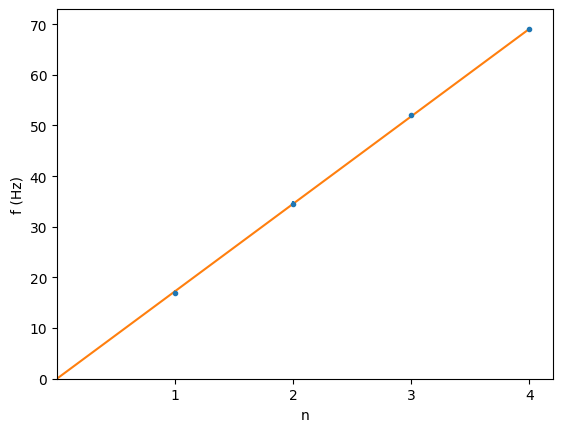
\includegraphics[width=0.8\textwidth]{Immagini/n.png}
    \caption{Interpolazione della frequenza in funzione del numero armonico con un parametro libero.}
\end{figure}

Il test del $\chi^2$ restituisce un $\Tilde{\chi}_o^2$=0.16, che per tre gradi di libertà corrisponde ad una probabilità del 92.6\%. Si conferma perciò la dipendenza lineare tra frequenza e numero armonico, in accordo con la relazione teorica:
\begin{equation}
  f_n = \frac{nv}{2L}  
  \label{eq:frequenze}
\end{equation}

Il coefficiente angolare interpolato è $k_{misurato} = \qty{17.27 \pm 0.09}{Hz}$, mentre quello ricavato dalla relazione 1 è $k_{teorico} = \qty{19.0 \pm 1.0}{Hz}$. Tramite un t-test  è  stata verificata la compatibilità di questi due valori, ottenendo una probabilità di accordo del 12.9\%, che corrisponde a un valore di $t_0 = 1.52$ ottenuto secondo la relazione:

\begin{equation}
t_0 = \frac{\abs{x_1-x_2}}{\sqrt{{\sigma}_{x_1}^2+{\sigma}_{x_2}^2}}
\label{t_test}
\end{equation}

 A partire da $k_{misurato}$, tramite la relazione \eqref{eq:frequenze}, si ottiene $v = \qty{22.7 \pm 0.5}{m/s}$. Tale valore si può confrontare con la velocità di propagazione teorica $v_{teorica} = \qty{24.7 \pm 1.2}{m/s}$, prevista dalla relazione:
\begin{equation}
  v = \sqrt{\frac{\tau}{\mu}} 
  \label{eq:velocità-propagazione}
\end{equation}

dove $\tau = mg$ rappresenta la tensione applicata alla corda e $\mu$ la massa lineare della stessa. Il t-test restituisce $t_0 = 1.54$, che indica una compatibilità del 12.4\% tra il valore osservato e quello atteso.

\section{Dipendenza della frequenza dalla tensione}

Successivamente è stata studiata la dipendenza della frequenza di risonanza  dalla tensione applicata alla corda per il secondo ordine di armonica.  
Mantenendo costante la lunghezza del tratto vibrante, sono state variate le masse appese al sistema di carrucola e supporto, modificando così la tensione della corda.

Le frequenze misurate sono riportate nella Tabella seguente:

\begin{table}[H]
\centering
\begin{tabular}{ccc}
\hline
Massa appesa (\unity{kg}) & Frequenza (\unit{Hz}) & Incertezza (\unit{Hz}) \\
\hline
0.13048 & 40.0 & 1.0 \\
0.08062 & 32.0 & 1.0 \\
0.09061 & 33.0 & 1.0 \\
0.11058 & 37.0 & 1.0 \\
0.15045 & 42.0 & 1.0 \\
0.18034 & 47.0 & 1.0 \\
0.28036 & 57.0 & 1.0 \\
0.38008 & 65.0 & 1.0 \\
\hline
\end{tabular}
\caption{Frequenze misurate al variare della tensione applicata alla corda.}
\end{table}

Secondo il modello teorico delle onde stazionarie su una corda tesa, la frequenza di risonanza di una data armonica dipende dalla radice quadrata della tensione. In particolare per la seconda armonica si ha
\begin{equation}
    f=\frac{1}{L} \sqrt{\frac{\tau}{\mu}}
    \label{eq:frequenza-t-variabile}
\end{equation}

Per verificare tale dipendenza è stato costruito il grafico della frequenza in funzione di $\sqrt{\tau}$ ed è stata effettuata un’interpolazione lineare tramite il metodo dei minimi quadrati.

\begin{figure}[H]
    \centering
    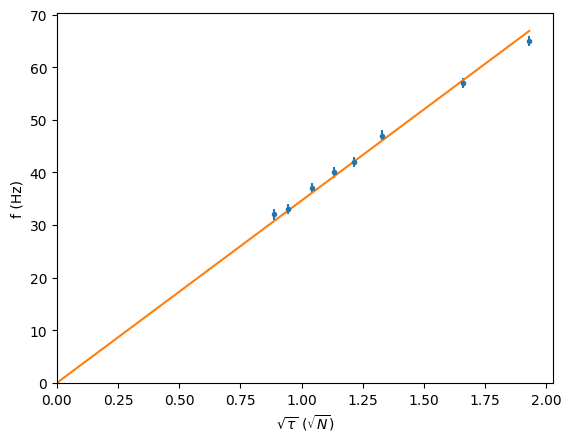
\includegraphics[width=0.8\textwidth]{Immagini/T.png}
    \caption{Dipendenza della frequenza dalla radice quadrata della tensione applicata alla corda.}
\end{figure}

Il grafico mostra una buona compatibilità con l’andamento lineare previsto teoricamente. Le piccole deviazioni osservate possono essere attribuite alle incertezze sperimentali sulle misure di frequenza, alla non perfetta rigidità dei vincoli e agli effetti dissipativi presenti nel sistema reale.

Dalla pendenza della retta interpolante è possibile ricavare una stima della velocità di propagazione delle onde sulla corda e confrontarla con il valore teorico ottenuto dalla relazione:

\[
v = \sqrt{\frac{\tau}{\mu}}
\]

dove $\mu$ rappresenta la massa lineare della corda.

Otteniamo dunque un valore del chi quadro ridotto di
$\Tilde{\chi_o^2}=1.0965$

Corrisponde a un p-value  di 0.36

\section{Dipendenza della frequenza dalla lunghezza del tratto di corda teso}

Nella terza parte dell’esperienza è stata studiata la dipendenza della frequenza di risonanza dalla lunghezza del tratto vibrante della corda.  
La tensione è stata mantenuta costante utilizzando una massa totale pari a $m = 0.28036\ \text{kg}$,
mentre è stata variata la lunghezza del tratto vibrante della corda.  
Le misure di frequenza sono state effettuate mantenendo fissata la stessa armonica e considerando un’incertezza strumentale pari a $\sigma_f = \qty{0.5}{Hz}$

Le lunghezze sono state misurate con un’incertezza:

\[
\sigma_L = 0.015\ \text{m}
\]

La massa della corda è risultata:

\[
m_{\text{corda}} = (5.22 \pm 0.05)\times10^{-3}\ \text{kg}
\]

mentre la massa lineare vale:

\[
\mu = 0.00210\ \text{kg/m}
\]

Le frequenze misurate al variare della lunghezza della corda sono riportate nella seguente tabella:

\begin{table}[H]
\centering
\begin{tabular}{ccc}
\hline
Lunghezza $L$ [m] & Frequenza $f$ [Hz] & Incertezza [Hz] \\
\hline
0.657 & 57.0 & 0.5 \\
0.822 & 46.0 & 0.5 \\
0.542 & 69.0 & 0.5 \\
0.411 & 92.0 & 0.5 \\
0.966 & 39.0 & 0.5 \\
1.123 & 33.0 & 0.5 \\
\hline
\end{tabular}
\caption{Frequenze misurate al variare della lunghezza del tratto vibrante della corda.}
\end{table}

Dal modello teorico delle onde stazionarie si prevede una dipendenza inversamente proporzionale tra frequenza e lunghezza della corda:

\[
f \propto \frac{1}{L}
\]

Per verificare tale relazione è stato costruito il grafico della frequenza in funzione dell’inverso della lunghezza armonica $\frac{1}{L_H}$ ed è stata effettuata un’interpolazione lineare tramite il metodo dei minimi quadrati.

\begin{figure}[H]
    \centering
    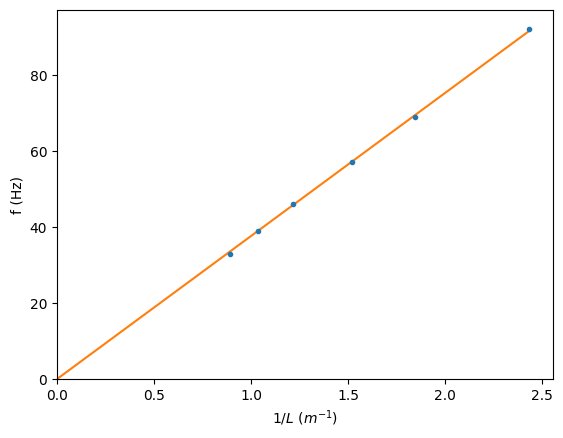
\includegraphics[width=0.8\textwidth]{Immagini/L.png}
    \caption{Andamento della frequenza in funzione dell’inverso della lunghezza del tratto vibrante della corda.}
\end{figure}
Il grafico mostra un andamento compatibile con la linearità prevista teoricamente. Le piccole deviazioni dalla retta interpolante possono essere attribuite alle incertezze sperimentali sulla misura della lunghezza del tratto vibrante, agli effetti dissipativi e alla non perfetta rigidità dei vincoli della corda.

Dalla pendenza della retta interpolante è possibile ricavare una stima della velocità di propagazione delle onde sulla corda e confrontarla con il valore teorico previsto dalla relazione:

\[
v = \sqrt{\frac{\tau}{\mu}}
\]

dove $\tau$ rappresenta la tensione applicata alla corda e $\mu$ la massa lineare della stessa.

Otteniamo dunque un valore del chi quadro ridotto di
$\Tilde{\chi_o^2}=0.608$

Corrisponde a un p-value di: 0.694

\section{Dipendenza della frequenza dalla massa lineare}

Nell’ultima parte dell’esperienza è stata studiata la dipendenza della frequenza di risonanza dalla massa lineare della corda.  
Per fare ciò sono state utilizzate corde differenti, caratterizzate da diversa massa e lunghezza, mantenendo costante la tensione applicata e fissando la lunghezza del tratto vibrante.

La massa totale applicata al sistema è stata mantenuta pari a:

\[
m = 0.28036\ \text{kg}
\]

mentre la lunghezza del tratto vibrante è stata fissata a:

\[
L = (0.697 \pm 0.020)\ \text{m}
\]

Le frequenze sono state misurate utilizzando sempre la stessa armonica e con un’incertezza strumentale pari a:

\[
\sigma_f = 0.5\ \text{Hz}
\]

Per ciascuna corda è stata calcolata la massa lineare secondo la relazione:

\[
\mu = \frac{m}{L}
\]

Le misure ottenute sono riportate nella seguente tabella:

\begin{table}[H]
\centering
\begin{tabular}{ccc}
\hline
Corda & Massa lineare $\mu$ [kg/m] & Frequenza $f$ [Hz] \\
\hline
Verde fluo & 0.002281 & 52.0 \\
Gialla e nera & 0.002368 & 51.0 \\
Nera & 0.002020 & 55.0 \\
Rossa & 0.002099 & 54.0 \\
\hline
\end{tabular}
\caption{Frequenze misurate per corde con diversa massa lineare.}
\end{table}

Dal modello teorico delle onde stazionarie su una corda tesa si prevede che la frequenza dipenda inversamente dalla radice quadrata della massa lineare:

\[
f \propto \frac{1}{\sqrt{\mu}}
\]

Per verificare tale relazione è stato costruito il grafico della frequenza in funzione di:

\[
\sqrt{\mu_n}
\]

ed è stata effettuata un’interpolazione lineare tramite il metodo dei minimi quadrati.

\begin{figure}[H]
    \centering
    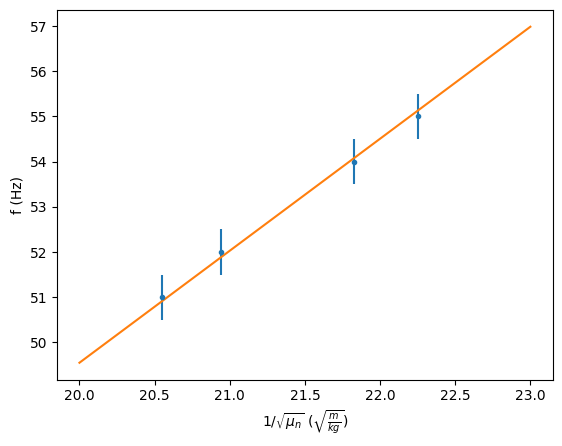
\includegraphics[width=0.8\textwidth]{Immagini/ML.png}
    \caption{Dipendenza della frequenza dalla radice quadrata della massa lineare della corda.}
\end{figure}
Il grafico mostra una compatibilità qualitativa con l’andamento teorico previsto. Le deviazioni osservate possono essere attribuite alle limitate differenze tra le masse lineari delle corde utilizzate, oltre che alle incertezze sperimentali sulla misura della frequenza, della lunghezza e della massa delle corde.

L'interpolazione lineare ha fornito:

\[
k_{\rm exp}=(2.478\pm0.012)
\]

mentre il valore teorico atteso risulta:

\[
k_{\rm teo}=(2.379\pm0.051)
\]

Il test di compatibilità tra i due valori fornisce

\[
|t|=1.88
\]

corrispondente a un p-value di circa il 6\%.

I due risultati risultano quindi compatibili entro il livello di significatività adottato, pur mostrando una lieve tensione statistica.


\section{Osservazioni}

Un eventuale allungamento della corda quando viene posta in trazione può influenzare le misure sperimentali in diversi modi.  
Nel nostro caso si è osservato sperimentalmente che la corda, quando viene tesa sulla macchina, può allungarsi di circa:

\[
\Delta L \simeq 7.2\ \text{mm}
\]

Tale effetto comporta innanzitutto una variazione della lunghezza effettiva del tratto vibrante della corda. Poiché la frequenza delle onde stazionarie dipende inversamente dalla lunghezza:

\[
f_n = \frac{nv}{2L}
\]

un aumento di $L$ produce una diminuzione della frequenza di risonanza rispetto al valore teorico atteso assumendo la corda perfettamente rigida.

Inoltre, l’allungamento modifica anche la massa lineare della corda. Infatti, a massa totale costante, un aumento della lunghezza comporta una lieve diminuzione della densità lineare:

\[
\mu = \frac{m}{L}
\]

e quindi una variazione della velocità di propagazione:

\[
v = \sqrt{\frac{\tau}{\mu}}
\]

Questo effetto tende ad aumentare leggermente la velocità dell’onda e quindi la frequenza. Tuttavia, nel nostro caso, la variazione della lunghezza del tratto vibrante rappresenta l’effetto dominante.

L’allungamento della corda può quindi introdurre una sistematica differenza tra valori teorici e sperimentali delle frequenze misurate, specialmente per tensioni elevate, e costituisce una possibile sorgente di errore sistematico nell’esperienza.
